\documentclass[conference]{IEEEtran}
\usepackage{cite}
\usepackage{amsmath,amssymb,amsfonts}
\usepackage{algorithmic}
\usepackage{graphicx}
\usepackage{textcomp}
\usepackage{xcolor}
\usepackage{booktabs}
\usepackage{multirow}
\usepackage{hyperref}
\usepackage{array}

\def\BibTeX{{\rm B\kern-.05em{\sc i\kern-.025em b}\kern-.08em
    T\kern-.1667em\lower.7ex\hbox{E}\kern-.125emX}}

\begin{document}

\title{Beyond Accuracy Drops: Characterizing How Vision-Language Model Hallucinations Shift Across Image Domains}

\author{\IEEEauthorblockN{Renuka Oladri}
\IEEEauthorblockA{Department of Computer Science\\
Email: shravya3003@gmail.com}}

\maketitle

\begin{abstract}
Vision-language models (VLMs) are widely known to hallucinate, but existing evaluations typically report aggregate accuracy on single-domain benchmarks, obscuring whether models fail \textit{differently} across image domains or merely at different rates. We introduce a unified probing framework that evaluates two open-source VLMs---LLaVA-1.5-7B and InternVL2-8B---across four visually distinct domains (natural photographs, data charts, medical radiographs, and mobile UI screenshots) using an identical six-category failure taxonomy. Our 945-probe evaluation reveals that domain shift does not simply degrade performance uniformly; rather, it reconfigures the failure profile in model-specific ways. LLaVA achieves 0\% accuracy on chart value extraction while fabricating plausible numbers, yet outperforms InternVL2 on medical existence detection. InternVL2 resists adversarial object hallucination at 86\% accuracy on charts where LLaVA collapses to 29\%. A chi-square interaction test confirms that failure-type distributions are significantly domain-dependent for both models ($p < 0.0001$). These results demonstrate that benchmarking VLM reliability requires domain-stratified evaluation across structured failure categories, not aggregate accuracy on a single domain.
\end{abstract}

\begin{IEEEkeywords}
vision-language models, hallucination, domain shift, VLM evaluation, multimodal reasoning
\end{IEEEkeywords}

\section{Introduction}

The deployment of vision-language models in domains beyond natural photography---radiology reading assistance, automated chart interpretation, UI accessibility tools---raises a practical question that current benchmarks do not answer: when a VLM trained predominantly on natural images encounters a chest X-ray or a stacked bar chart, does it simply get worse at everything, or does it break in fundamentally different ways?

Prior work on VLM hallucination has established that models confidently assert the presence of absent objects \cite{li2023pope}, fabricate spatial relationships \cite{liu2023hallusionbench}, and generate plausible but unsupported descriptions \cite{rohrbach2018object}. However, these studies typically operate within a single image domain, making it impossible to distinguish domain-general weaknesses (e.g., a tendency toward affirmative responses) from domain-specific capability gaps (e.g., inability to parse chart axes).

The few cross-domain evaluations that exist---MME \cite{fu2023mme}, MMMU \cite{yue2023mmmu}---use different question formats, answer distributions, and annotation protocols per domain, confounding the image domain with the evaluation methodology. A model scoring lower on medical VQA than on natural-image VQA may be struggling with the images, the question phrasing, or the shift in answer distribution.

We address this confound directly. Our contribution is a unified probing framework where the \textit{same} six failure categories---existence, attribute, count, spatial, OCR/numeric, and confabulation---are tested using identically structured probes across four image domains sourced from established datasets with reliable ground truth. This design isolates the effect of the image domain from confounds introduced by evaluation methodology.

We evaluate LLaVA-1.5-7B \cite{liu2023llava15} and InternVL2-8B \cite{chen2024internvl}, two architecturally distinct open-source VLMs, on 945 probes spanning 185 images. Our analysis focuses on the \textit{domain $\times$ category interaction}---whether the distribution of failure types changes across domains---rather than aggregate accuracy.

\section{Related Work}

\subsection{Object Hallucination in VLMs}

POPE \cite{li2023pope} introduced adversarial polling for object existence, demonstrating that VLMs hallucinate objects that frequently co-occur with those actually present. Rohrbach et al. \cite{rohrbach2018object} quantified object hallucination in image captioning, finding that models mention objects absent from the scene at rates exceeding 10\%. CHAIR \cite{rohrbach2018object} provided a metric for this, but remains limited to COCO object categories.

\subsection{Multi-Domain VLM Benchmarks}

MME \cite{fu2023mme} evaluates 14 perception and cognition subtasks but uses heterogeneous question formats across domains. MMMU \cite{yue2023mmmu} tests college-level reasoning across disciplines but conflates domain knowledge gaps with visual hallucination. HallusionBench \cite{liu2023hallusionbench} focuses on visual illusions and manipulated images rather than domain shift. None of these isolate the image domain as the independent variable while holding the evaluation protocol constant.

\subsection{Domain-Specific VLM Evaluation}

Medical VQA benchmarks like SLAKE \cite{liu2021slake} and VQA-RAD \cite{lau2018vqarad} test within the medical domain but do not compare against non-medical performance. ChartQA \cite{masry2022chartqa} evaluates chart understanding but does not map failures to a taxonomy comparable with object-hallucination work. Our framework bridges these isolated evaluations by applying a shared taxonomy across all four domains.

\section{Methodology}

\subsection{Design Rationale}

The central methodological requirement is that any observed difference in failure patterns across domains must be attributable to the image domain, not to differences in question format, answer distribution, or ground-truth annotation quality. We achieve this through three controls:

\begin{enumerate}
\item \textbf{Shared taxonomy}: Every probe belongs to one of six categories (Table~\ref{tab:taxonomy}), defined identically across domains.
\item \textbf{Uniform question structure}: Probes within each category follow the same syntactic pattern regardless of domain (e.g., ``Is there a [X] in this image?'' for existence).
\item \textbf{Closed-form grading}: Five of six categories use exact-match or numeric-tolerance grading against ground truth derived from source dataset annotations. No LLM-as-judge is used for the primary results.
\end{enumerate}

\subsection{Domains and Datasets}

We draw images from four established datasets, selected for reliable ground-truth annotations:

\begin{itemize}
\item \textbf{Natural (COCO val2017)}: 50 images with instance segmentation annotations providing object categories, counts, and bounding box positions.
\item \textbf{Chart (ChartQA)}: 45 multi-column chart images with underlying data tables providing exact numeric values and category labels.
\item \textbf{Medical (SLAKE)}: 45 radiology images with organ segmentation masks, semantic labels, and structured VQA pairs.
\item \textbf{Screenshot (ScreenQA/RICO)}: 45 mobile UI screenshots with annotated UI element bounding boxes and text labels.
\end{itemize}

\subsection{Failure Taxonomy}

\begin{table}[t]
\caption{Failure taxonomy applied uniformly across domains}
\label{tab:taxonomy}
\centering
\small
\begin{tabular}{@{}lll@{}}
\toprule
Category & Tests & Grading \\
\midrule
Existence & Is X present? & Exact (yes/no) \\
Attribute & Color/size/shape of X & Exact + forced-choice \\
Count & How many X? & Exact (integer) \\
Spatial & X left/right of Y? & Exact (yes/no) \\
OCR/Numeric & Read a value & Tolerance ($\pm$0.1) \\
Confabulation & Open description & Manual review \\
\bottomrule
\end{tabular}
\end{table}

\subsection{Probe Construction}

For each image, we generate 4--6 probes from the source dataset's ground-truth metadata. Key design decisions include:

\textbf{Adversarial existence negatives.} Following the POPE protocol \cite{li2023pope}, negative existence probes ask about objects that are \textit{absent} but frequently co-occur with objects that \textit{are} present, based on a co-occurrence matrix computed over the full dataset.

\textbf{Balanced spatial polarity.} Each spatial probe is paired with its negation (swapping the spatial relation) to produce equal numbers of yes/no ground truths, preventing a model from achieving high accuracy through response bias alone.

\textbf{Forced-choice attribute parsing.} For comparative attribute questions (``Which is bigger, X or Y?''), we parse the model's response using regex patterns that identify comparative constructions (``the X is bigger than Y''), resolving cases where both options appear in the response.

The final probe set contains 945 probes: 274 natural, 282 chart, 218 medical, and 171 screenshot.

\subsection{Model Configuration}

Both models are evaluated under identical inference conditions:

\begin{itemize}
\item \textbf{LLaVA-1.5-7B} \cite{liu2023llava15}: fp16 precision, greedy decoding, max 200 tokens. Loaded via \texttt{LlavaForConditionalGeneration}.
\item \textbf{InternVL2-8B} \cite{chen2024internvl}: bf16 precision, greedy decoding, max 200 tokens. Dynamic image tiling (up to 12 tiles). Loaded via \texttt{AutoModel} with \texttt{trust\_remote\_code}.
\end{itemize}

No quantization is applied. Both models run on a single NVIDIA A40 (48GB). The absence of stochastic decoding ensures exact reproducibility given the same random seed for probe generation.

\subsection{Response Parsing and Grading}

Model responses are parsed by category-specific regex extractors. For existence and spatial probes, we detect affirmative/negative keywords with word-boundary matching. For count probes, we extract the first integer. For OCR/numeric, we prioritize percentage and currency patterns before falling back to generic number extraction, with year values from the question excluded to prevent echo-matching.

Grading is exact-match for existence, attribute, count, and spatial categories. OCR/numeric uses a tolerance of $\pm$0.1 after stripping currency and percentage symbols. Confabulation probes return the raw response for manual review and are excluded from accuracy calculations.

Unparseable responses (2.0\% for LLaVA, 4.9\% for InternVL2) are excluded from accuracy calculations. All raw responses are preserved for reproducibility.

\section{Results}

\subsection{Overall Domain-Level Performance}

\begin{table}[t]
\caption{Overall accuracy by domain (\%)}
\label{tab:domain_overall}
\centering
\small
\begin{tabular}{@{}lcc@{}}
\toprule
Domain & LLaVA-1.5-7B & InternVL2-8B \\
\midrule
Natural (COCO) & 68.3 & 83.3 \\
Chart (ChartQA) & 51.1 & 83.1 \\
Medical (SLAKE) & 53.4 & 47.3 \\
Screenshot (RICO) & 61.9 & 79.4 \\
\bottomrule
\end{tabular}
\end{table}

Table~\ref{tab:domain_overall} shows that InternVL2 substantially outperforms LLaVA on three of four domains, with gaps of 15--32 percentage points on natural, chart, and screenshot images. However, this pattern reverses on medical images, where LLaVA achieves 53.4\% compared to InternVL2's 47.3\%. This reversal is the first indication that domain shift affects models asymmetrically.

\subsection{Domain $\times$ Category Accuracy}

\begin{table*}[t]
\caption{Accuracy (\%) by domain and failure category. Dashes indicate categories with no probes for that domain. Bold indicates the higher-scoring model per cell.}
\label{tab:main_results}
\centering
\small
\begin{tabular}{@{}ll*{2}{c}c*{2}{c}c*{2}{c}c*{2}{c}@{}}
\toprule
& & \multicolumn{2}{c}{Existence} & & \multicolumn{2}{c}{Attribute} & & \multicolumn{2}{c}{Count} & & \multicolumn{2}{c}{Spatial} \\
\cmidrule{3-4} \cmidrule{6-7} \cmidrule{9-10} \cmidrule{12-13}
Domain & OCR & LLaVA & IV2 & & LLaVA & IV2 & & LLaVA & IV2 & & LLaVA & IV2 \\
\midrule
Natural & --- & 85.0 & \textbf{93.9} & & --- & --- & & 40.4 & \textbf{75.0} & & 63.5 & \textbf{73.0} \\
Chart & 0.0/\textbf{71.1} & 71.2 & \textbf{93.2} & & 77.4 & \textbf{83.9} & & 51.1 & \textbf{77.8} & & 48.8 & \textbf{83.7} \\
Medical & --- & \textbf{60.9} & 50.9 & & \textbf{44.4} & 33.3 & & \textbf{48.9} & 42.6 & & 56.3 & \textbf{85.7} \\
Screenshot & --- & 67.9 & \textbf{92.3} & & --- & --- & & --- & --- & & 52.1 & \textbf{58.3} \\
\bottomrule
\end{tabular}
\end{table*}

Table~\ref{tab:main_results} presents the central result. Several patterns emerge that aggregate accuracy conceals:

\textbf{Chart OCR capability gap.} LLaVA scores 0\% on chart OCR/numeric probes (0 of 43 correct). Inspection of raw responses reveals that LLaVA does not refuse to answer; instead, it generates fabricated values (e.g., responding ``\$1,000,000'' when the ground truth is ``79.3''). InternVL2 achieves 71.1\% on the same probes, demonstrating a qualitative capability difference rather than a quantitative one.

\textbf{Medical reversal.} LLaVA outperforms InternVL2 on medical existence (60.9\% vs 50.9\%), attribute (44.4\% vs 33.3\%), and count (48.9\% vs 42.6\%). InternVL2's stronger general performance does not transfer to medical images and in fact inverts. This suggests that InternVL2's larger visual vocabulary may introduce more confident but incorrect responses on out-of-distribution medical imagery.

\textbf{Spatial yes-bias.} Fig.~\ref{fig:spatial} reveals that LLaVA achieves near-perfect accuracy on spatial probes where the ground truth is ``yes'' (92--100\%) but collapses to 0--35\% where the ground truth is ``no.'' The model defaults to affirming any spatial relationship it is asked about. InternVL2 shows more balanced spatial reasoning, though screenshot spatial accuracy on negative cases reaches only 50\%.

\subsection{Adversarial Existence Analysis}

\begin{table}[t]
\caption{Existence accuracy (\%) by distractor type}
\label{tab:adversarial}
\centering
\small
\begin{tabular}{@{}llcccc@{}}
\toprule
& & \multicolumn{2}{c}{LLaVA} & \multicolumn{2}{c}{InternVL2} \\
\cmidrule(lr){3-4} \cmidrule(lr){5-6}
Domain & & Pos. & Adv. & Pos. & Adv. \\
\midrule
Natural & & 94.0 & 76.0 & 92.0 & 95.9 \\
Chart & & 97.8 & 28.6 & 97.8 & 85.7 \\
Screenshot & & 75.6 & 57.6 & 97.8 & 84.8 \\
\bottomrule
\end{tabular}
\end{table}

Table~\ref{tab:adversarial} separates existence probes by whether the queried object is genuinely present (positive) or a plausible-but-absent co-occurring entity (adversarial). The most striking result is LLaVA's chart adversarial accuracy of 28.6\%---the model affirms the presence of chart categories that do not exist 71.4\% of the time. InternVL2 maintains 85.7\% accuracy on the same adversarial probes.

LLaVA's yes-bias is domain-dependent: it says ``yes'' 88\% of the time on chart existence probes but only 59\% on natural photos. InternVL2 shows a more uniform yes-rate (48--66\% across domains), suggesting better-calibrated confidence.

\subsection{Statistical Validation}

We test whether the distribution of error types across categories differs by domain using a chi-square test of independence, computed separately for each model. The contingency table has domains as rows and error counts per category as columns.

\begin{itemize}
\item \textbf{LLaVA}: $\chi^2 = 172.12$, $p < 0.0001$, $df = 12$
\item \textbf{InternVL2}: $\chi^2 = 131.87$, $p < 0.0001$, $df = 12$
\end{itemize}

Both tests reject the null hypothesis that failure-type distributions are independent of domain. The models do not simply get worse on out-of-domain images; they fail in categorically different ways.

\begin{figure}[t]
\centering
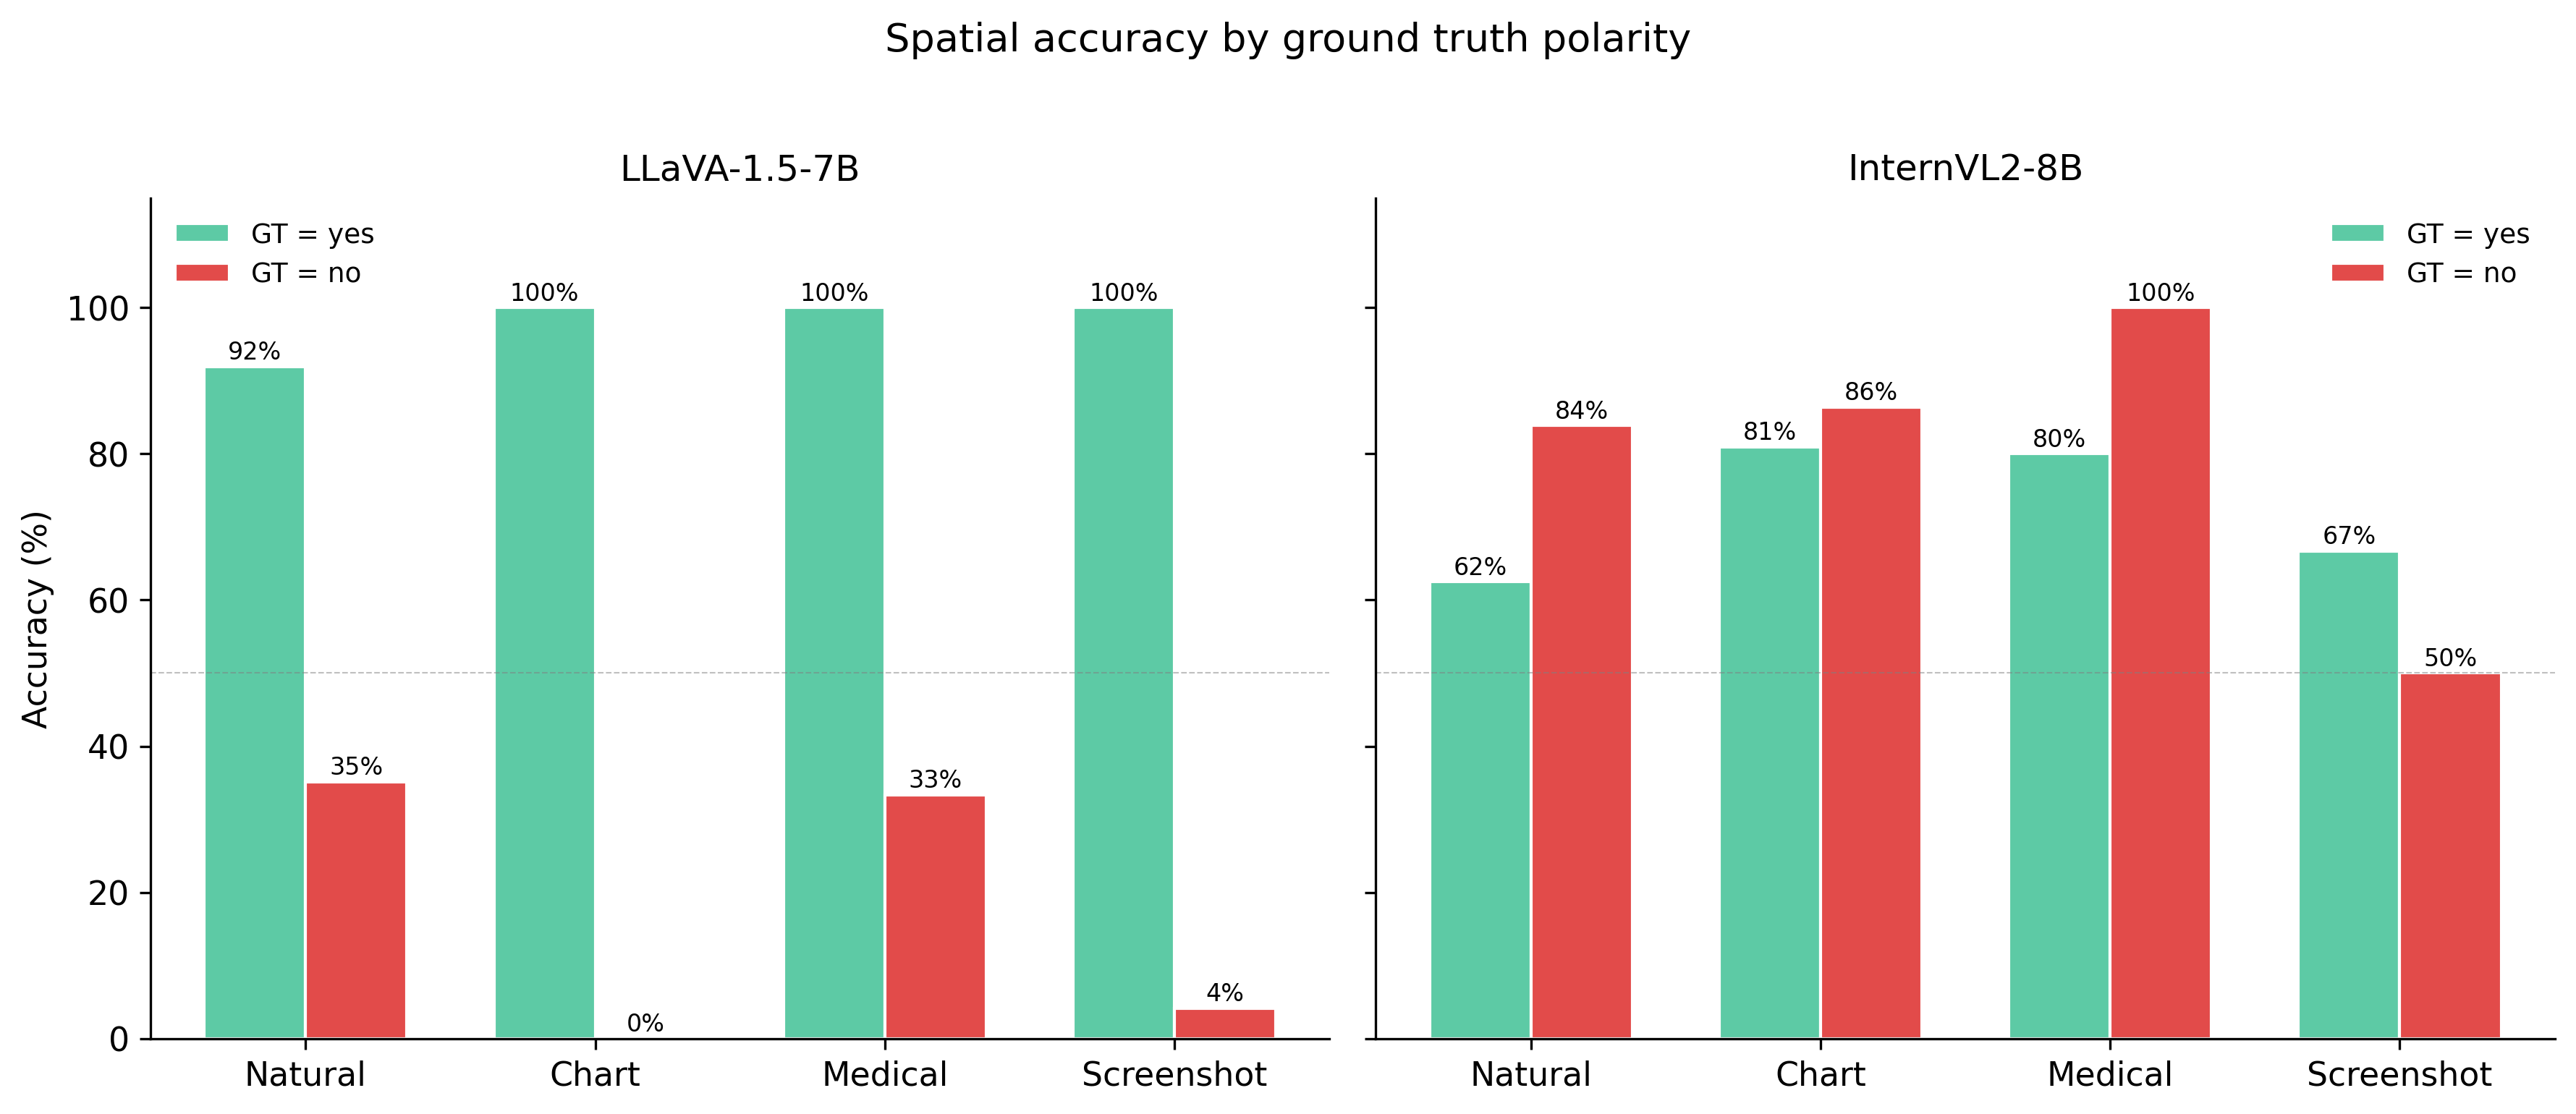
\includegraphics[width=\columnwidth]{figures/fig6_spatial_balance.png}
\caption{Spatial accuracy by ground truth polarity. LLaVA exhibits extreme yes-bias (100\% on GT=yes, 0--35\% on GT=no). InternVL2 is more balanced but still shows polarity-dependent accuracy on screenshots.}
\label{fig:spatial}
\end{figure}

\begin{figure}[t]
\centering
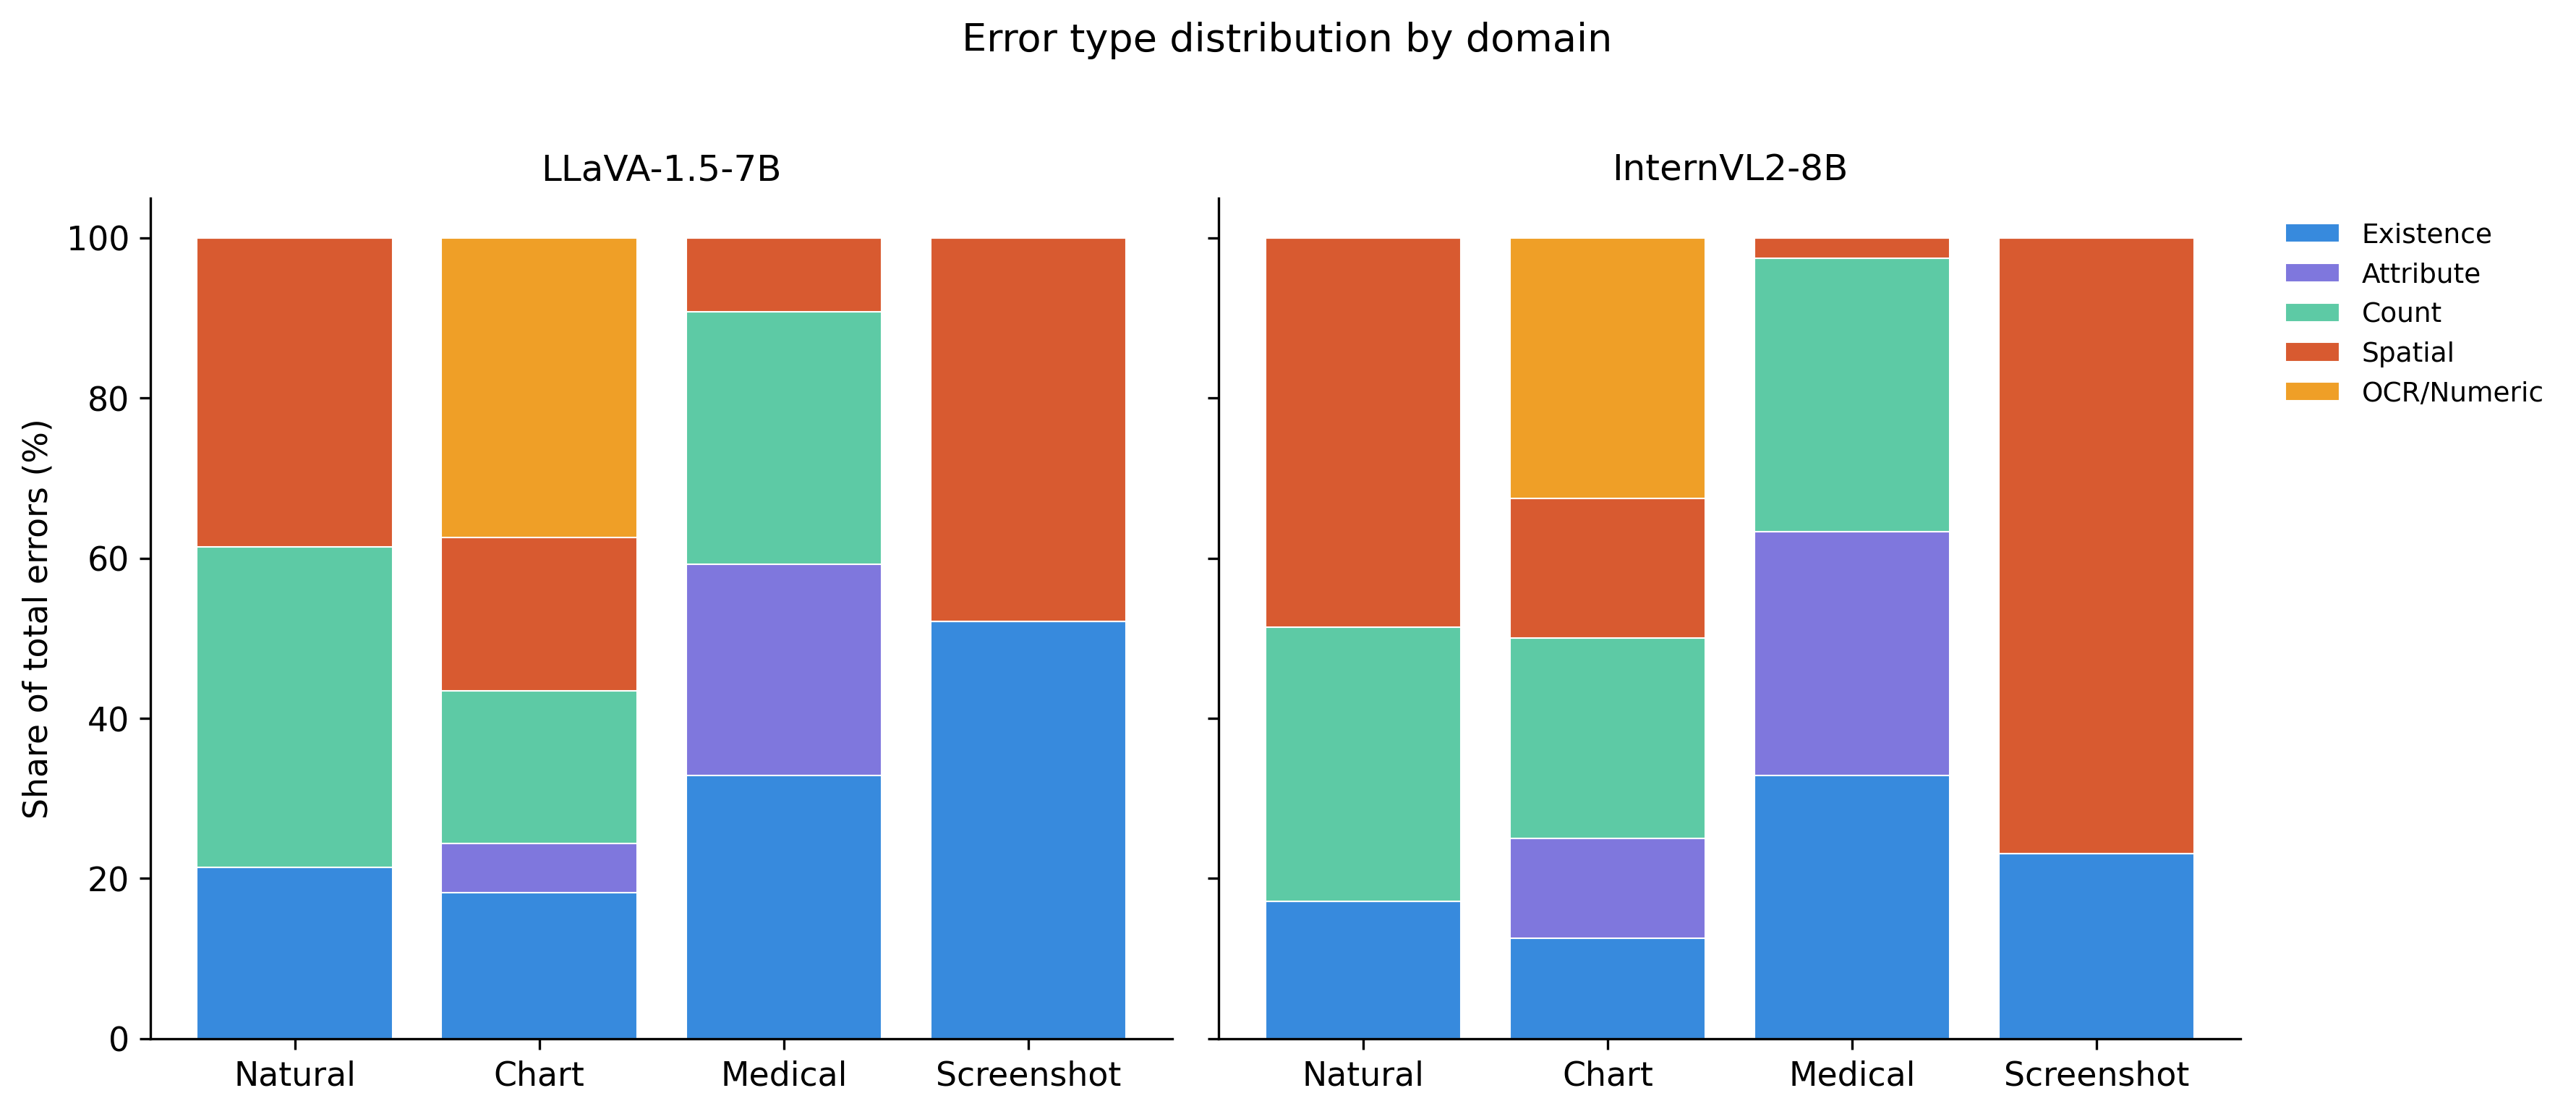
\includegraphics[width=\columnwidth]{figures/fig5_error_profile.png}
\caption{Normalized error-type distribution by domain. Chart errors for LLaVA are dominated by OCR failures (37\% of errors). Medical errors are distributed across categories for both models. Screenshot errors are dominated by spatial and existence failures.}
\label{fig:error_profile}
\end{figure}

\subsection{Error Profile Analysis}

Fig.~\ref{fig:error_profile} shows the normalized distribution of error types per domain. For LLaVA, chart errors are dominated by OCR/numeric failures (37\% of all chart errors), a category that contributes zero errors to natural and medical domains. This demonstrates that the chart domain does not amplify existing weaknesses---it introduces an entirely new failure mode.

For InternVL2, the error profile shifts from count-dominated on natural images (41\% of natural errors) to attribute-dominated on medical images (30\% of medical errors). The failure composition changes across domains even though overall accuracy is more stable.

\section{Discussion}

\subsection{Implications for VLM Deployment}

The medical reversal---where InternVL2's superior general capability becomes a liability---has practical implications for deployment decisions. A model that performs best on aggregate benchmarks may not be the safest choice for a specific domain. Domain-specific evaluation using the taxonomy we propose would identify that InternVL2's medical existence accuracy (50.9\%) falls below the 60.9\% achieved by the smaller LLaVA model.

\subsection{Yes-Bias as a Domain-Modulated Phenomenon}

The spatial yes-bias results (Fig.~\ref{fig:spatial}) suggest that the commonly observed affirmative bias in VLMs \cite{li2023pope} is not a fixed model property but varies with image domain. LLaVA's yes-rate ranges from 59\% (natural) to 88\% (chart), indicating that unfamiliar visual contexts amplify the bias. This has methodological implications: evaluations that do not balance ground-truth polarity will overestimate spatial and existence capabilities, particularly on out-of-domain images.

\subsection{Limitations}

Our study has several limitations that should be noted. First, the probe set uses 45--50 images per domain, which is sufficient for detecting large effects (as evidenced by $p < 0.0001$) but may miss subtler patterns. Second, not all categories have probes in all domains: natural images lack attribute and OCR probes, screenshots lack count and attribute probes, and medical images lack OCR probes. These gaps reflect genuine limitations of the source datasets rather than methodological oversights. Third, the SLAKE medical probes use the dataset's native QA pairs rather than our adversarial co-occurrence protocol, which means medical existence results are not directly comparable to other domains' adversarial probes. Fourth, we evaluate two models at a single parameter scale (7--8B); extending to larger models and additional architectures would strengthen generalizability claims.

\section{Conclusion}

We have demonstrated that domain shift in VLMs is not merely an accuracy degradation phenomenon but a qualitative reconfiguration of failure patterns. The same model that completely fails at reading chart values may outperform a stronger competitor on medical image interpretation. The same spatial reasoning capability that appears robust on natural photos collapses to random chance when tested with balanced polarity probes.

These findings argue for a shift in VLM evaluation practice: from single-domain aggregate accuracy toward domain-stratified, category-resolved failure analysis. The probing framework, evaluation pipeline, and all results presented here are publicly available to support this transition.

\bibliographystyle{IEEEtran}

\begin{thebibliography}{10}

\bibitem{li2023pope}
Y.~Li, Y.~Du, K.~Zhou, J.~Wang, W.~X. Zhao, and J.-R. Wen, ``Evaluating object hallucination in large vision-language models,'' in \textit{Proc. EMNLP}, 2023, pp. 292--305.

\bibitem{liu2023hallusionbench}
F.~Guan, K.~Liu, Q.~Xie, Y.~Zhu, and Y.~Yang, ``HallusionBench: An advanced diagnostic suite for entangled language hallucination and visual illusion in large vision-language models,'' in \textit{Proc. CVPR}, 2024.

\bibitem{rohrbach2018object}
A.~Rohrbach, L.~A. Hendricks, K.~Burns, T.~Darrell, and K.~Saenko, ``Object hallucination in image captioning,'' in \textit{Proc. EMNLP}, 2018, pp. 4035--4045.

\bibitem{fu2023mme}
C.~Fu, P.~Chen, Y.~Shen, Y.~Qin, M.~Zhang, X.~Lin, J.~Yang, X.~Zheng, K.~Li, X.~Sun, Y.~Wu, and R.~Ji, ``MME: A comprehensive evaluation benchmark for multimodal large language models,'' \textit{arXiv preprint arXiv:2306.13394}, 2023.

\bibitem{yue2023mmmu}
X.~Yue, Y.~Ni, K.~Zhang, T.~Zheng, R.~Liu, G.~Zhang, S.~Stevens, D.~Jiang, W.~Ren, Y.~Sun, C.~Wei, B.~Yu, R.~Yuan, R.~Sun, M.~Yin, B.~Zheng, Z.~Yang, J.~Liu, W.~Huang, H.~Sun, Y.~Su, and W.~Chen, ``MMMU: A massive multi-discipline multimodal understanding and reasoning benchmark for expert AGI,'' in \textit{Proc. CVPR}, 2024.

\bibitem{liu2023llava15}
H.~Liu, C.~Li, Y.~Li, and Y.~J. Lee, ``Improved baselines with visual instruction tuning,'' in \textit{Proc. CVPR}, 2024.

\bibitem{chen2024internvl}
Z.~Chen, J.~Wu, W.~Wang, W.~Su, G.~Chen, S.~Xing, Z.~Muyan, Q.~Zhang, X.~Zhu, L.~Lu, B.~Li, P.~Luo, T.~Lu, Y.~Qiao, and J.~Dai, ``InternVL: Scaling up vision foundation models and aligning for generic visual-linguistic tasks,'' in \textit{Proc. CVPR}, 2024.

\bibitem{liu2021slake}
B.~Liu, L.-M. Zhan, L.~Xu, L.~Ma, Y.~Yang, and X.-M. Wu, ``SLAKE: A semantically-labeled knowledge-enhanced dataset for medical visual question answering,'' in \textit{Proc. ISBI}, 2021, pp. 1650--1654.

\bibitem{lau2018vqarad}
J.~J. Lau, S.~Gayen, A.~Ben~Abacha, and D.~Demner-Fushman, ``A dataset of clinically generated visual questions and answers about radiology images,'' \textit{Scientific Data}, vol.~5, no. 180251, 2018.

\bibitem{masry2022chartqa}
A.~Masry, D.~X. Long, J.~Q. Tan, S.~Joty, and E.~Hoque, ``ChartQA: A benchmark for question answering about charts with visual and logical reasoning,'' in \textit{Proc. ACL Findings}, 2022, pp. 2263--2279.

\end{thebibliography}

\end{document}
